\documentclass[a4paper,11pt]{article}
\usepackage[english,polish]{babel}
\usepackage{polski}
\usepackage[utf8]{inputenc}
\usepackage{graphicx}
\usepackage{listings}
\usepackage{color}
\usepackage{amsmath}
\newcommand{\HRule}{\rule{\linewidth}{0.5mm}}
\begin{document}
\begin{titlepage}
    \begin{center}
        
\includegraphics[width=0.4\textwidth]{images/logo.jpg} \\[1cm]
        \textsc{\LARGE Systemy Czasu Rzeczywistego} \\[0.8cm]
        \textsc{\LARGE Dokumentacja Projektowa} \\[0.5cm]
        \HRule \\[0.4cm]
        { \huge \bfseries Winda Towarowa} \\[0.4cm]
        \HRule \\[1.5cm]
    
    \begin{minipage}{0.4\textwidth}
        \begin{flushleft} \large
        \emph{Autorzy:} \\
        Michał \textsc{Janiec} \\
        Bartosz \textsc{Polnik}
        \end{flushleft}
    \end{minipage}
    \begin{minipage}{0.4\textwidth}
        \begin{flushright} \large
            \emph{Prowadzący:} \\
            Dr. Inż. Michał \textsc{Turek}
        \end{flushright}
    \end{minipage}

    \vfill

    {\large \today}

    \end{center}
\end{titlepage}

\section{Wprowadzenie}
    Projekt został zrealizowany w ramach zajęć z przedmiotu Systemy Czasu Rzeczywistego.
    Jego celem jest zaznajomienie się z zagadnieniem tworzenia systemów czasu rzeczywistego w środowisku IBM Rational Rhapsody.
    Realizowanym przez nas przykładem jest winda towarowa. 


\section{Przedstawienie problemu}

    Winda towarowa to urządzenie stosowane w przemyśle. 
    Jest szeroko stosowana w kopalniach, halach produkcyjnych czy restauracjach.
    Zastosowanie jest proste: Na jednym z pięter pracownik
    przywołuje windę, ładuje towar, a następnie wysyła windę na inne piętro, gdzie ktoś inny odbiera towar.
    W przeciwieństwie do windy osobowo towarowej nie przewozi się wewnątrz osób co prowadzi do kilku uproszczeń;
    Sterowanie windą odbywa się w całości przy pomocy paneli sterowniczych znajdujących się na zewnątrz windy. 
    Ponadto nie ma potrzeby stosowania automatycznie otwieranych drzwiczek. 
    Konieczne jest także zachowanie wszelkich norm bezpieczeństwa: winda dba o zachowanie odpowiedniej prędkości podczas wznoszenia i opuszczania,  jak i odpowiedniej wagi załadunku.
    Ponadto jak większość urządzeń przemysłowych 
    windy towarowe często posiadają tak zwany kill switch - przycisk pozwalający na natychmiastowe wyłączenie urządenia. 
   
    \begin{center} 
    	
\includegraphics{images/elevator.png} \\Pewna winda towarowa. Na panelu widoczny czerwony przycisk "kill switch"\\ 
    \end{center} 
    
\section{Wymagania}
    \subsection{Wymagania funkcjonalne}
    	\begin{itemize}
    		\item przemieszczanie towarów między piętrami
    	\end{itemize}
    \subsection{Wymagania niefunkcjonalne}
    	\begin{itemize}
    		\item niezawodnść - brak przerw w działaniu a także poprawne zachowanie w sutacjach brzegowych
    		 (np. gdy po wznowieniu zasilania winda znajduje się między piętrami)
    		\item bezpieczeństwo - wykrywanie przeciążeń, niezamkniętych drzwiczek, możliwość natychmiastowego wyłączenia urządzenia 
    		\item prosty interfejs użytkownika - pozwoli uniknąć pomyłek - zwiększy bezpieczeństwo
    	\end{itemize}
    	
\section{Przypadki użycia}
	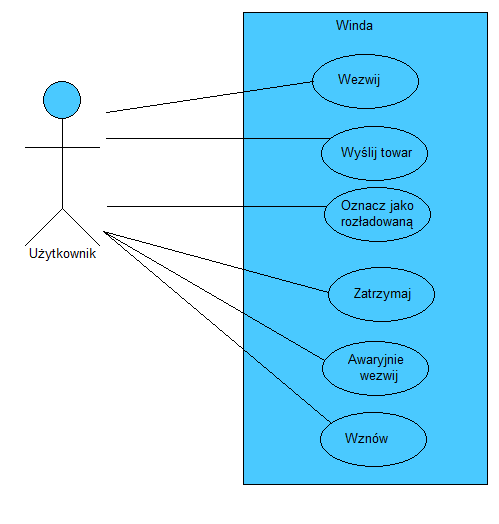
\includegraphics{images/useCase.png}    	
	\textbf{Scenariusze} \\
	\begin{itemize}
		\item Wezwij windę
		\begin{itemize}
			\item warunek wstępny - winda nie jest w stanie emergency
			\item warunek końcowy - winda znajduje się na piętrze wzywającego
			\item przebieg główny:
			\begin{itemize}
				\item użytkownik wciska przycisk \textbf{bring here},
				\item użytkownik czeka.
			\end{itemize}
		\end{itemize}
		\item Wyślij windę
		\begin{itemize}
			\item warunek wstępny - winda jest na tym samym piętrze co użytkownik, nie jest przeciążona, a drzwiczki są zamknięte
			\item warunek końcowy - winda znajduje się na piętre na które została wysłana
			\item przebieg główny:
			\begin{itemize}
				\item użytkownik wciska przycisk z numerem piętra
				\item użytkownik czeka.
			\end{itemize}
		\end{itemize}
		\item Oznacz windę jako rozładowaną - scenariusz podstawowy
		\begin{itemize}
			\item warunek wstępny - winda jest na tym samym piętrze co użytkownik, nie jest przeciążona, a drzwiczki są zamknięte
			\item warunek końcowy - winda może zostać wezwana przez kogoś innego
			\item przebieg główny:
			\begin{itemize}
				\item użytkownik wciska przycisk \textbf{ready},
			\end{itemize}
	
		\end{itemize}

		\item Zatrzymaj 
		\begin{itemize}
			\item warunek wstępny - brak,
			\item warunek końcowy - winda się zatrzymuje
			\item przebieg główny:
			\begin{itemize}
				\item użtkownik wciska przycisk \textbf{stop},
			\end{itemize}
		\end{itemize}
		
		\item Wezwij awaryjnie
		\begin{itemize}
			\item warunek wstępny - brak.
			\item warunek końcowy: Winda znajduje się na parterze
			\item przebieg główny:
			\begin{itemize}			
				\item użytkonik wciska przycisk \textbf{Emergency Bring Here},
			\end{itemize}
		\end{itemize}
		
		\item Wznów
		\begin{itemize}
			\item warunek wstępny - winda jest w stanie emergency,
			\item warunek końcowy - winda oczekuje na wezwania
			\item przebieg główny:
			\begin{itemize}
				\item użytkownik wciska przycisk \textbf{Emergency ready},
			\end{itemize}
		\end{itemize}
		
	\end{itemize}
    
\section{Architektura}
	Winda została zaprojektowan jako maszyna stanowa. \\	
	Winda posiada detektory:
	\begin{itemize}
		\item detektor stanu drzwiczek (otwarte/zamknięte)
		\item detektor obciążenia windy
	\end{itemize}
	a także efektor:
	\begin{itemize}
		\item silnik windy - przemieszczanie góra / dół
	\end{itemize}

	Uproszczony diagram stanów \\
	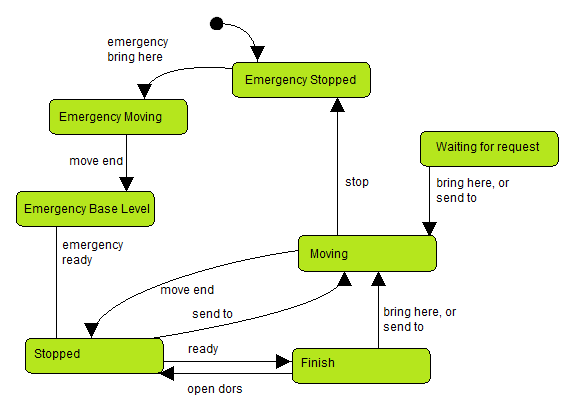
\includegraphics{images/simplifiedStateChart.png}
	
\section{Interfejs graficzny}
	\subsection{Interfejs wewnętrzy Rhapsody}
	   
	\begin{center} 
    		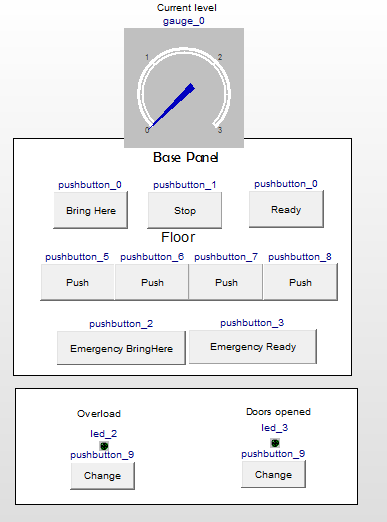
\includegraphics{images/rGuiBase.PNG} \\Interfejs na parterze\\ 
  	\end{center} 
  	
  	Wskazówka na górze pokazuje numer piętra. Na samym dole znajdują się diody informujące o tym czy drzwiczki są otwarte, oraz
  	czy winda jest przeciążona. Jeśli chcemy zasymulować zmiane jednego z tych parametrów wystarczy kliknąć na przycisku change pod spodem.
  	Środkowa część panelu to główny panel sterowniczy. Zawiera on przyciski  \textbf{Bring here} do wzywania windy, \textbf{Stop}
  	do zatrzymania, \textbf{Ready} dozakończenia akcji. Cztery przyciski poniżej służą do wysyłania na odpowiednie piętro.
  	 Natomiast przyciski emergecy służą do obsługi stanu emergency.
    

    		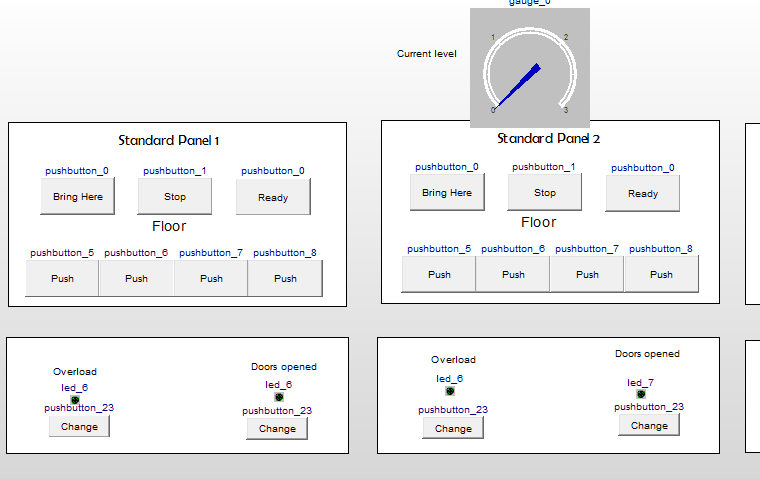
\includegraphics{images/rGuiStd.PNG} Interfejsy na pozostałych piętrach (interfejs 3 piętra nie widoczny)
  	
  	
  	Panele na pozostałych piętrach są bardzo zbliżone. Nie posiadają jedynie przycisków \textbf{Emergency Bring Here, Emergency Ready}.
  	
  	
  	
  	
  	Przykład urzycia windy.
  	
  	Po uruchomieniu winda jest w stanie \textbf{Emergency Stopped}. Aby móc ją używać należy wcisnąć przycisk \textbf{Emergency Ready}.
  	Winda jest gotowa do użytku. Teraz można kolejkować dla niej zadania.
  	Aby rozpocząć zadanie należy na dowolnym piętrze wcisnąć \textbf{Bring here}. Winda podjedzie na odpowiednie piętro.
  	Tam można ją załadować. Następnie posyłamy windę na odpowiednie piętro, gdzie może być rozładowana. 
  	Po rozładowaniu klikamy \textbf{Ready} i winda jest gotowa do przetworzenia następnego wezwania.

    
	\subsection{Interfejs zewnętrzny}
	\begin{center} 
    		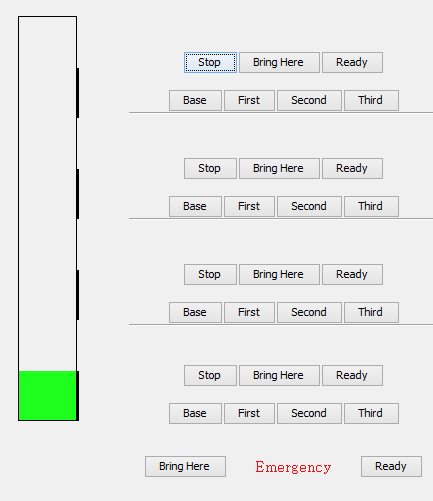
\includegraphics{images/oGui.PNG} \\Interfejsy zewnętrzny\\ 
  	\end{center} 
  	
  	Interfejs jest "odbiciem" tego z Rhapsody z tą różnicą że bardziej czytelnie prezentuje stan windy. Różni się także sposób otwierania 
  	drzwiczek i przeciążania windy. W celu przeciążenia windy wystarczy kliknąć jej rysunek (kolor odwzorowuje stan). W celu otwarcia drzwi 
  	wystarczy kliknąć na ich rysunek.

	
	
	
\section{Testy}
	Podczas testowania windy należy zwrócić uwagę na wszelkie sytuacje wyjątkowe.
	
	\subsection{Uruchomienie windy}
		\begin{enumerate}
			\item Próba wezwania windy na pierwszym piętrze
			\item Winda nie poinna się poruszyć
			\item Wciśnięcie przycisku \textbf{Emergency Ready}
			\item Próba wezwania windy na pierwszym piętrze 
			\item Winda powinna podjechać na pierwsze piętro
		\end{enumerate}
	\subsection{Załadunek windy}
		Warunek początkowy - winda jest poprawnie uruchomiona (przycisk Emergency Ready został już wciśnięty) - znajduje się na piętrze 0
		\begin{enumerate}
			\item Wciśnięcie bring here na parterze
			\item Otwarcie drzwiczek,
			\item Próba wysłania windy na następne piętro,
			\item Winda nie powinna się poruszyć
			\item Zwiększenie obciążenia powyżej progu,
			\item Zamknięcie drzwiczek
			\item Próba wysłania windy na następne piętro 
			\item Winda nie powinna się poruszyć
			\item Zdjęcie ciężaru poniżej limitu
			\item Próba wysłania windy na następne piętro
			\item Winda powinna pojechać			
		\end{enumerate}
	\subsection{Wzywanie windy i oznaczanie jako rozładowanej} 
		Warunek początkowy - winda jest poprawnie uruchomiona, znajduje się na poziomie 0
		\begin{enumerate}
			\item wciśnięcie przycisku \textbf{bring here} na pierwszym piętrze
			\item winda powinna przyjechać na pierwsze piętro
			\item wciśnięcie przycisku \textbf{bring here} na poziomie 0
			\item winda nie powinna podjechać (powinna czekać na rozładowanie)
			\item wciśnięcie przycisku \textbf{Second} na pierwszym poziomie
			\item winda powinna podjechać na drugie piętro
			\item wciścięcie przycisku \textbf{ready} na drugim piętrze
			\item winda powina rozpocząć kolejne zadanie (zjechać na poziom 0)
		\end{enumerate}
		
	\subsection{Przycisk stop i Emergency Ready}
		Warunek początkowy - winda jest poprawnie uruchomiona, znajduje się na poziomie 0
		\begin{enumerate}
			\item wciśnięcie przycisku stop
			\item próba wysłania windy na pierwsze piętro
			\item próba przywołania windy na pierszym piętrze 
			\item winda nie powinna się poruszyć
			\item przyciśnięcie przycisku \textbf{Emergency Ready}
			\item próba przywołania windy na pierszym piętrze 
			\item winda powinna się pojechać
			\item wciśnięcie przycisku stop, gdy winda znajduje się między piętrami.
			\item winda powinna się zatrzmać
		\end{enumerate} 
		
	\subsection{Przycisk EmergencyBringHere}
		\begin{enumerate}
			\item pozostawnienie windy między piętrami (opisane w poprzednim teście)
			\item wciśnięcie przycisku \textbf{Emergency Bring Here}
			\item winda powinna zjechać na dolne piętro
		\end{enumerate}
		
	
\section{Podsumowanie}
	Budowa oprogramowania przy pomocy środowiska IBM Rhapsody 
	okazała się ciekawym i bardzo rozwijającym doświadczeniem.
	Produkt firmy IBM umożliwia modelowanie systemów przy pomocy różnorodnych diagramów, najważniejszym dla nas
	typem diagramu jest diagram stanów, który pozwala definiować i nazywać pewne momenty w czasie życia systemu oraz określać przejścia pomiędzy nimi.
	Dzięki możliwości wizunej budowy i analizy systemów opartych o maszyny stanowe pakiet ten idalnie 
	nadaje się do budowy systemów czasu rzeczywistego, zapewniając wysoką przejżystość, pozwala unikać błędów i budować niezawodne oprogramowanie.
	Kolejnyą zaletą Rhapsody jest zastosowanie 
	języków C++ oraz Java które są powszechnie znane i posiadają bardzo 
	duże wsparcie technicze i ogromne ilości bibliotek.
	Dzięki IBM Raphsody udało nam się stosunkow szybko stworzyć funkcjonalny i stabilny projekt.






\end{document}
